\documentclass{beamer}
\usetheme{Berlin}
\usefonttheme[onlymath]{serif}
\setbeamertemplate{footline}[frame number]

\usepackage{xcolor}
\usepackage{graphicx}
\usepackage{amsmath,amsfonts,amssymb}
\usepackage{bm}
\setcounter{MaxMatrixCols}{20}
\usepackage{booktabs,array,multicol}
\usepackage{tikz}
\usetikzlibrary{arrows.meta,positioning,shapes}

\definecolor{myblue}{rgb}{0.0,0.0,0.7}
\setbeamercolor{item}{fg=myblue}
\setbeamercolor{block title}{bg=myblue,fg=white}
\setbeamercolor{block body}{bg=blue!7,fg=black}
\setbeamercolor{itemize item}{fg=myblue}
\setbeamercolor{custom top bar}{bg=black,fg=white}
\setbeamercolor{custom sub bar}{bg=myblue,fg=white}
\setbeamertemplate{navigation symbols}{}

\setbeamertemplate{background}{
  \begin{tikzpicture}[overlay,remember picture]
    \node[opacity=0.07,rotate=30] at (current page.center) {
      \begin{minipage}{\paperwidth}\centering
      {\color{blue!80!black}\Large\bfseries Automatic GFL/GFM Mode Switching}\\[0.15cm]
      {\color{blue!60!black}\large\bfseries PSDSC Center KMITL}
      \end{minipage}};
  \end{tikzpicture}
}
\setbeamertemplate{headline}{
  \leavevmode
  \hbox{\begin{beamercolorbox}[wd=\paperwidth,ht=3ex,dp=1.2ex,left]{custom top bar}
    \hspace*{2ex}\textbf{POWER SYSTEM DYNAMICS, STABILITY, AND CONTROL (PSDSC) RESEARCH CENTER}
  \end{beamercolorbox}}
  \vskip0pt
  \hbox{\begin{beamercolorbox}[wd=\paperwidth,ht=2.5ex,dp=1ex]{custom sub bar}
    \hspace*{4ex}\raisebox{0.1ex}{\rule{0.8pt}{1.5ex}\rule{1.5ex}{0.8pt}}\hspace*{1ex}\insertsection
    \hfill Automatic GFL/GFM Mode Switching\hspace*{2ex}
  \end{beamercolorbox}}
}

\title{\large\textbf{Automatic GFL/GFM Mode Switching}}
\author{Mr. Phichitchai Jueajan (66010569)\\Mr. Pakkapol Phdungdan (66010612)\\[0.2cm]
Advisor: Dr. Tossaporn Surinkaew}
\institute{Department of Electrical Engineering, Faculty of Engineering\\
King Mongkut's Institute of Technology Ladkrabang (KMITL)}
\date{}
\titlegraphic{
\includegraphics[width=0.95in]{figures/images.png}}
\newcommand{\pu}{\,\mathrm{p.u.}}

\begin{document}

\begin{frame}[plain]
  \titlepage
\end{frame}

\begin{frame}{Table of Contents}
  \begin{multicols}{2}
    \tableofcontents
  \end{multicols}
\end{frame}
\section{Introduction}
\begin{frame}{Introduction}
\begin{columns}[c,onlytextwidth]
\column{0.55\textwidth}
\small
\begin{itemize}
  \item Increasing IBR penetration reduces reliance on synchronous generation.
  \item GFL converters require an external voltage-angle reference.
  \item GFM converters can establish voltage and frequency in weak-grid or islanded operation.
  \item This project studies automatic GFL/GFM switching in an IEEE 14-bus system with one SG and four dual-mode IBRs.
\end{itemize}
\column{0.42\textwidth}
\centering
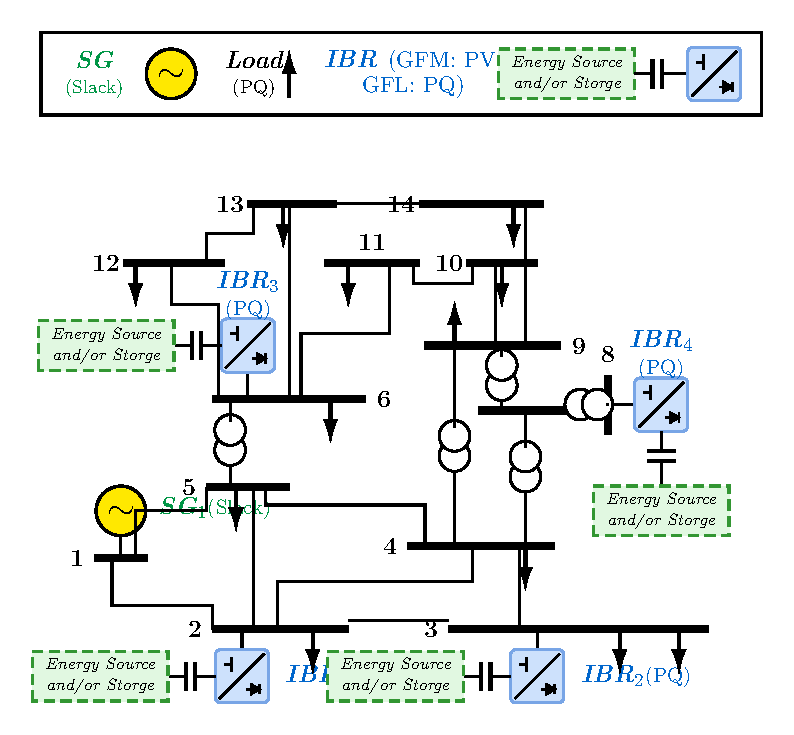
\includegraphics[width=0.80\linewidth]{figures/ieee14_dual_mode_ibr_diagram.pdf}
\vspace{0.15cm}
\footnotesize
\textbf{Research focus:} maintain a valid grid reference after SG loss and return support after SG recovery.
\end{columns}
\end{frame}

\section{Objectives}
\begin{frame}{Project Objectives}
\begin{columns}[c,onlytextwidth]
\column{0.58\textwidth}
\small
\begin{enumerate}
  \item Develop an in-house analysis chain for Power Flow, SSSA, and Time-Domain Simulation.
  \item Model four IBRs that can operate in either GFL or GFM mode.
  \item Select and switch GFM support according to the system condition.
  \item Verify switching, island operation, and synchronous-generator reconnection under one disturbance chronology.
\end{enumerate}
\column{0.39\textwidth}
\centering
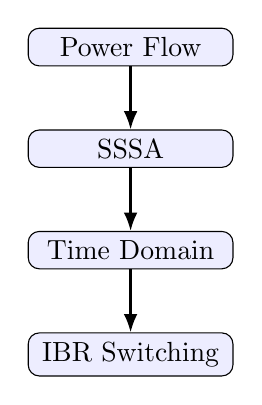
\begin{tikzpicture}[node distance=8mm,>=Latex]
\node[draw,rounded corners,fill=blue!7,minimum width=2.6cm] (pf) {Power Flow};
\node[draw,rounded corners,fill=blue!7,below=of pf,minimum width=2.6cm] (sssa) {SSSA};
\node[draw,rounded corners,fill=blue!7,below=of sssa,minimum width=2.6cm] (ts) {Time Domain};
\node[draw,rounded corners,fill=blue!7,below=of ts,minimum width=2.6cm] (sw) {IBR Switching};
\draw[->,thick] (pf)--(sssa); \draw[->,thick] (sssa)--(ts); \draw[->,thick] (ts)--(sw);
\end{tikzpicture}
\end{columns}
\end{frame}
\section{Study System}
\begin{frame}{Study System: IEEE 14-Bus with 1 SG + 4 IBRs}
\begin{columns}[c,onlytextwidth]
\column{0.50\textwidth}
\small
\begin{itemize}
  \item SG1 at bus 1 provides the normal grid reference.
  \item Dual-mode IBRs are connected at buses 2, 3, 6, and 8.
  \item Each IBR supports \textbf{GFL}, \textbf{GFM}, and tripped states.
  \item The network equations are shared by PF, SSSA, and TS.
\end{itemize}
\vspace{0.3cm}
\[
\boxed{\;\bm{g}(\bm{x},\bm{y})=\bm{Y}_{\!net}\bm{V}-\bm{I}_{inj}(\bm{x},\bm{V})=\bm{0}\;}
\]
\column{0.47\textwidth}
\centering
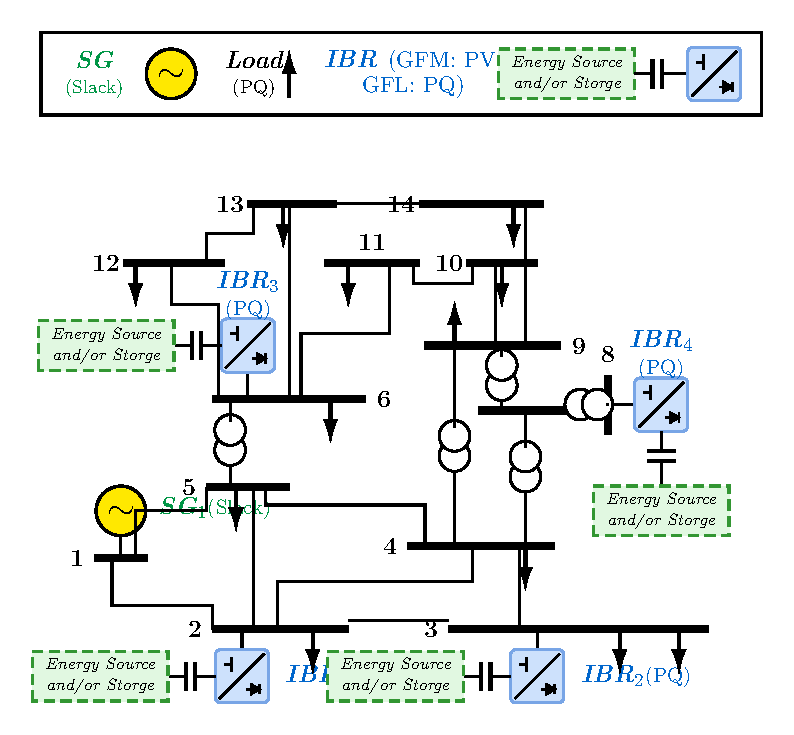
\includegraphics[width=0.84\linewidth]{figures/ieee14_dual_mode_ibr_diagram.pdf}
\end{columns}
\end{frame}

\section{Power Flow}
\begin{frame}{Power Flow Formulation}
\begin{columns}[c,onlytextwidth]
\column{0.54\textwidth}
\small
For bus $i$,
\begin{align*}
P_i &= V_i\sum_{k=1}^{n}V_k\left(G_{ik}\cos\theta_{ik}+B_{ik}\sin\theta_{ik}\right),\\
Q_i &= V_i\sum_{k=1}^{n}V_k\left(G_{ik}\sin\theta_{ik}-B_{ik}\cos\theta_{ik}\right).
\end{align*}
Newton--Raphson iteration:
\[
\boxed{\bm{J}_{PF}(\bm{z}^{(r)})\Delta\bm{z}^{(r)}=-\bm{F}_{PF}(\bm{z}^{(r)})}
\]
\[
\boxed{\bm{z}^{(r+1)}=\bm{z}^{(r)}+\Delta\bm{z}^{(r)}}
\]
\column{0.43\textwidth}
\small
\begin{block}{Bus constraints}
\begin{tabular}{lll}
\toprule
Bus & Specified & Solved \\
\midrule
REF & $|V|,\theta$ & $P,Q$ \\
PV  & $P,|V|$ & $Q,\theta$ \\
PQ  & $P,Q$ & $|V|,\theta$ \\
\bottomrule
\end{tabular}
\end{block}
\vspace{0.25cm}
\centering
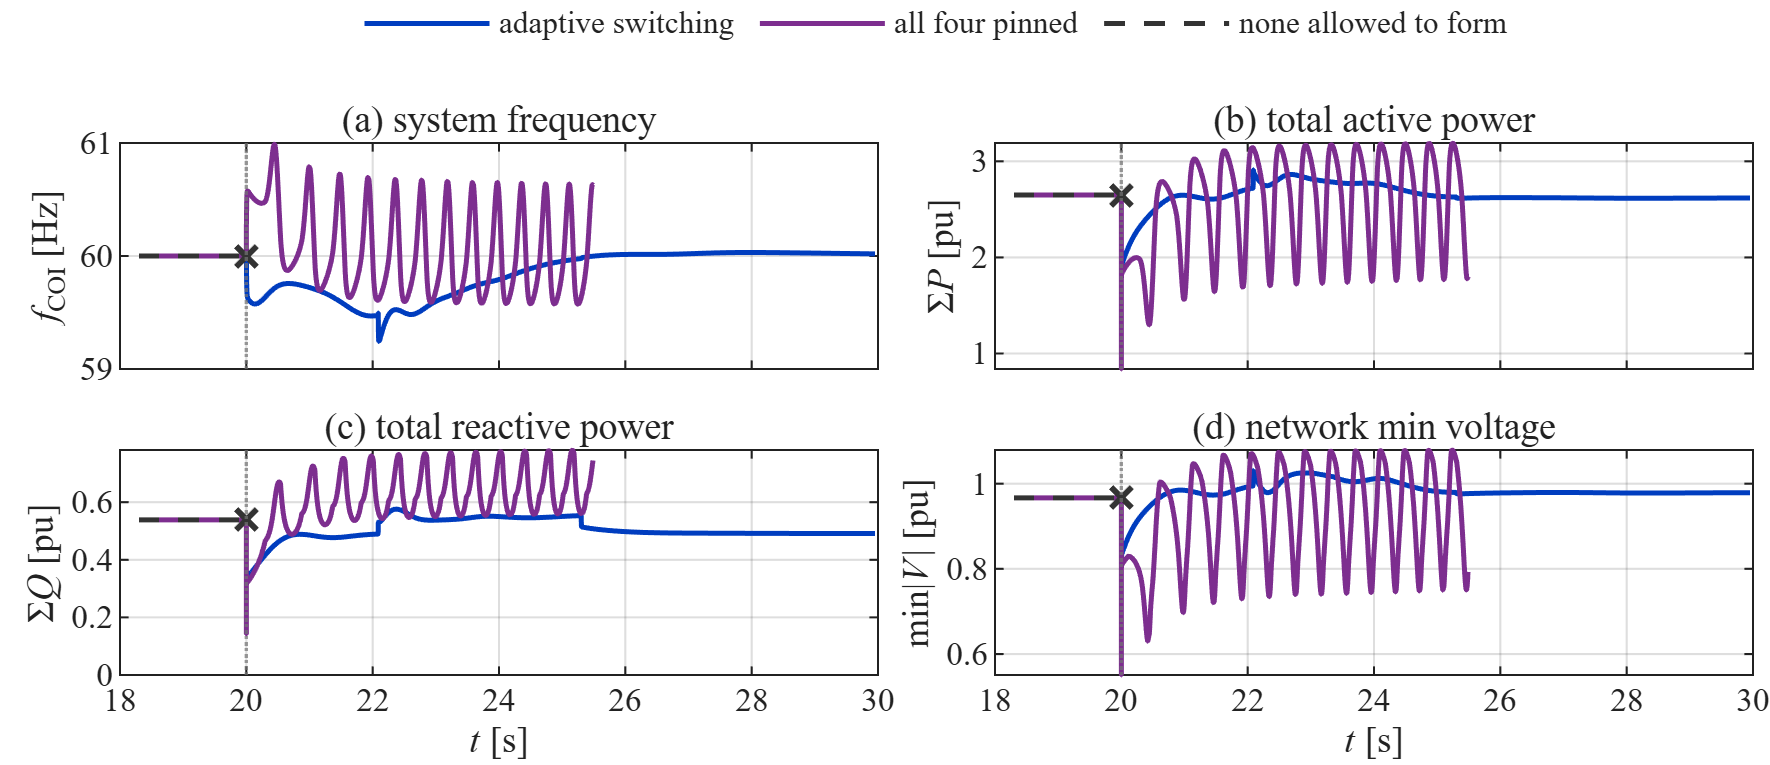
\includegraphics[width=0.92\linewidth]{figures/presentation_pf_sssa_ts_gfm/slide_necessity.png}
\end{columns}
\end{frame}
\section{Small-Signal Stability}
\begin{frame}{Small-Signal Stability Analysis (SSSA)}
\begin{columns}[c,onlytextwidth]
\column{0.55\textwidth}
\small
Nonlinear DAE:
\[
\dot{\bm{x}}=\bm{f}(\bm{x},\bm{y}),\qquad
\bm{0}=\bm{g}(\bm{x},\bm{y})
\]
Linearization around $(\bm{x}_0,\bm{y}_0)$:
\[
\begin{bmatrix}\Delta\dot{\bm{x}}\\\bm{0}\end{bmatrix}=
\begin{bmatrix}\bm{f}_x&\bm{f}_y\\\bm{g}_x&\bm{g}_y\end{bmatrix}
\begin{bmatrix}\Delta\bm{x}\\\Delta\bm{y}\end{bmatrix}
\]
Eliminating algebraic variables:
\[
\boxed{\bm{A}=\bm{f}_x-\bm{f}_y(\bm{g}_y\backslash\bm{g}_x)}
\]
\column{0.42\textwidth}
\small
\[
\boxed{\bm{A}\bm{v}=\lambda\bm{v}}
\]
\[
f=\frac{|\operatorname{Im}\lambda|}{2\pi},\qquad
\zeta=-\frac{\operatorname{Re}\lambda}{|\lambda|}
\]
\begin{block}{Stability criterion}
$\operatorname{Re}(\lambda)<0$ for all physical modes; the selector also checks the declared damping-ratio floor.
\end{block}
\end{columns}
\end{frame}
\section{Time-Domain Simulation}
\begin{frame}{Time-Domain Simulation (TS)}
\begin{columns}[c,onlytextwidth]
\column{0.56\textwidth}
\small
\[ \dot{\bm{x}}=\bm{f}(\bm{x},\bm{y}),\qquad \bm{0}=\bm{g}(\bm{x},\bm{y}) \]
\textbf{Implicit trapezoidal step}
\begin{align*}
\bm{R}_x &= \bm{x}_{n+1}-\bm{x}_{n}-\frac{h}{2}(\bm{f}_{n}+\bm{f}_{n+1})=\bm{0},\\
\bm{R}_y &= \bm{g}(\bm{x}_{n+1},\bm{y}_{n+1})=\bm{0},\\
\boxed{\bm{J}_R\Delta\bm{z}}&=\boxed{-\bm{R}},\qquad \bm{z}=[\bm{x};\bm{y}].
\end{align*}
\column{0.41\textwidth}
\small
\begin{block}{Event handling}
\begin{itemize}
  \item Exact landing on event times
  \item Preserve the left-limit state
  \item Atomic mode/topology transaction
  \item Right-limit KCL must converge
  \item Roll back a rejected transaction
\end{itemize}
\end{block}
\end{columns}
\end{frame}
\section{IBR Dynamic Model}
\begin{frame}{Dual-Mode IBR State Representation}
\begin{columns}[c,onlytextwidth]
\column{0.56\textwidth}
\footnotesize
Each converter uses a fixed 17-coordinate superset:
\[
\boxed{\bm{x}_{IBR}=\begin{bmatrix}\bm{x}_{p}^{T}&\bm{x}_{GFL}^{T}&\bm{x}_{GFM}^{T}&I_{dc}\end{bmatrix}^{T}}
\]
\begin{align*}
\bm{x}_{p}&=[i_d\;i_q\;V_{dc}]^T,\\
\bm{x}_{GFL}&=[\delta_{PLL}\;\xi_{PLL}\;\xi_P\;\xi_Q\;\xi_{Id}\;\xi_{Iq}]^T,\\
\bm{x}_{GFM}&=[\delta_{VSG}\;\omega_{VSG}\;E\;\xi_{Vd}\;\xi_{Vq}\;\xi_{Id}^{GFM}\;\xi_{Iq}^{GFM}]^T.
\end{align*}
\[
\mathcal{A}_{GFL}=\{1{:}9,17\},\qquad
\mathcal{A}_{GFM}=\{1{:}3,10{:}17\}.
\]
\column{0.41\textwidth}
\centering
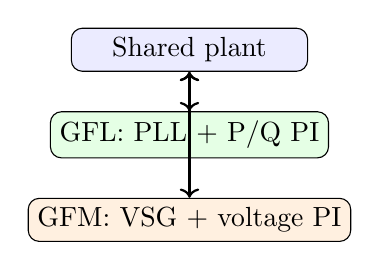
\begin{tikzpicture}[node distance=5mm]
\node[draw,rounded corners,fill=blue!8,minimum width=3.0cm] (p) {Shared plant};
\node[draw,rounded corners,fill=green!10,below=of p,minimum width=3.0cm] (gfl) {GFL: PLL + P/Q PI};
\node[draw,rounded corners,fill=orange!12,below=of gfl,minimum width=3.0cm] (gfm) {GFM: VSG + voltage PI};
\draw[<->,thick] (p)--(gfl); \draw[<->,thick] (p)--(gfm);
\end{tikzpicture}
\vspace{0.25cm}
\begin{block}{Mode rule}
Only the selected controller branch evolves; inactive controller states are held.
\end{block}
\end{columns}
\end{frame}
\begin{frame}{GFL and GFM State Equations}
\begin{columns}[t,onlytextwidth]
\column{0.49\textwidth}
\footnotesize
\textbf{Grid-Following (GFL)}
\begin{align*}
\dot{\delta}_{PLL}&=k_{p,PLL}v_q+k_{i,PLL}\xi_{PLL},\\
\dot{\xi}_{PLL}&=v_q,\\
e_P&=\kappa P^{\star}-P,\\ e_Q&=\kappa Q^{\star}-Q,\\
i_d^{\star}&=k_{pP}e_P+k_{iP}\xi_P,\\
i_q^{\star}&=-(k_{pQ}e_Q+k_{iQ}\xi_Q).
\end{align*}
\centering\textit{PLL-synchronized current control}
\column{0.49\textwidth}
\footnotesize
\textbf{Grid-Forming (GFM)}
\begin{align*}
M\dot{\omega}&=\kappa P^{\star}-P-D_v(\omega-1),\\
\dot{\delta}_{VSG}&=\omega_b(\omega-1),\\
\tau_E\dot E&=k_Q(\kappa Q^{\star}-Q)-k_E(E-E^{\star}),\\
e_{vd}&=E-v_d,\qquad e_{vq}=-v_q,\\
i_d^{\star}&=k_{pV}e_{vd}+k_{iV}\xi_{Vd},\\
i_q^{\star}&=k_{pV}e_{vq}+k_{iV}\xi_{Vq}.
\end{align*}
\centering\textit{VSG establishes angle and frequency}
\end{columns}
\end{frame}
\section{IBR Mode Switching}
\begin{frame}{Automatic GFL/GFM Switching Law}
\begin{columns}[c,onlytextwidth]
\column{0.56\textwidth}
\footnotesize
\textbf{Severity index}
\begin{align*}
J_V&=\frac{\bigl||V_i|-V_i^{\star}\bigr|}{0.10\pu},\\
J_f&=\frac{|f_{COI}-60|}{0.50\,\mathrm{Hz}},\\
S&=\operatorname{sat}_{[0,1]}\!\left(0.5J_V+0.5J_f\right).
\end{align*}
\textbf{Mode command}
\[
q^+=\begin{cases}
\mathrm{GFM},&S\ge0.65\quad(0.10\,\mathrm{s}),\\
\mathrm{GFL},&S<0.35\quad(1.00\,\mathrm{s}),\\
q,&\text{otherwise}.
\end{cases}
\]
\column{0.41\textwidth}
\small
\begin{block}{Switch transaction}
\[
\boxed{\left\|I^{+}-I^{-}\right\|_{\infty}\le10^{-10}\pu}
\]
\begin{itemize}
  \item Equilibrium + SSSA certified candidate
  \item Target states initialized at the present terminal point
  \item Right-limit KCL converges before commit
\end{itemize}
\end{block}
\end{columns}
\end{frame}

\IfFileExists{figures/switch_ieee14_decision/run_summary_v2.tex}{% Generated by generate_ieee14_report_scalars. Do not edit.
%
% PROVENANCE. Accepted values of output/diagnostics/ieee14_gfm_lock_compare_dcreal/adaptive_250s.mat.
% Produced by run_ieee14_gfm_lock_comparison, whose option set is the
% flagship driver's plus agsi_reference=true (opt-in, post-processing only).
% This cache is NOT bit-identical to the earlier delivered artifact, and no
% such claim is made for it: the DC-link closure changed under
% NUM-2026-08-20-01, so the trajectory legitimately differs. Compare it to
% the earlier cache by outcome, never by bit-identity.
% No value here is rounded, scaled, smoothed or otherwise altered.
%
% Regenerate with:  pf_init_paths; generate_ieee14_report_scalars(result_file="output/diagnostics/ieee14_gfm_lock_compare_dcreal/adaptive_250s.mat")

\newcommand{\NewRunEnd}{250.000}
\newcommand{\NewRunVMin}{0.036855}
\newcommand{\NewRunVMax}{1.523183}
\newcommand{\NewRunFMin}{58.838795}
\newcommand{\NewRunFMax}{61.138560}
\newcommand{\NewRunSubdivision}{0}
\newcommand{\NewRunDomainRejects}{584}
\newcommand{\NewRunResidual}{$9.9596\times10^{-9}$}
\newcommand{\NewRunReclose}{159.240}
\newcommand{\NewRunRecloseStatus}{SUCCESS}
\newcommand{\NewRunSyncDV}{0.008785}
\newcommand{\NewRunSyncDF}{$6.4601\times10^{-13}$}
\newcommand{\NewRunSyncDTheta}{5.015017}
\newcommand{\NewRunFirstRelease}{25.310}
\newcommand{\NewRunReleaseOne}{25.310}
\newcommand{\NewRunReleaseTwo}{146.247}
\newcommand{\NewRunReleaseThree}{152.390}
\newcommand{\NewRunReleaseFour}{--}
\newcommand{\NewRunAugmentOne}{22.052}
\newcommand{\NewRunAugmentTwo}{51.333}
\newcommand{\NewRunAugmentThree}{53.372}
\newcommand{\NewRunAugmentFour}{148.267}
\newcommand{\NewRunNRelease}{3}
\newcommand{\NewRunNAugment}{4}
\newcommand{\NewRunGfmMax}{4}
\newcommand{\NewRunSamples}{4990}
\newcommand{\NewRunRejectedSteps}{135}
\newcommand{\NewRunTerminalF}{60.000000}
\newcommand{\NewRunTerminalVMin}{0.9667}
\newcommand{\NewRunTerminalVMax}{1.0575}
\newcommand{\NewRunStepper}{adaptive}
\newcommand{\NewRunReselection}{NO\_FEASIBLE\_SG\_ON\_ONE\_STEP}
}{}
\IfFileExists{figures/switch_ieee14_decision/comparison_macros.tex}{% Generated by generate_ieee14_gfm_lock_comparison. Do not edit.
% Every number the comparison section prints comes from here, so the prose cannot drift
% from the runs. Arm keys: adaptive, pinned_gfm1, pinned_gfm2, pinned_gfm4, locked_gfl

\newcommand{\ArmAdaptiveLabel}{adaptive}
\newcommand{\ArmAdaptiveHorizon}{250.000}
\newcommand{\ArmAdaptiveConverged}{1}
\newcommand{\ArmAdaptiveReclose}{159.2397}
\newcommand{\ArmAdaptiveGfmMax}{4}
\newcommand{\ArmAdaptiveFailure}{--}
\newcommand{\ArmAdaptiveSamples}{4990}
\newcommand{\ArmAdaptiveRejected}{135}
\newcommand{\DfAdaptiveSGtrip}{0.7587}
\newcommand{\SetAdaptiveSGtrip}{0.0041}
\newcommand{\DfAdaptiveLoadstep}{1.0035}
\newcommand{\SetAdaptiveLoadstep}{0.3753}
\newcommand{\DfAdaptiveFault}{1.1386}
\newcommand{\SetAdaptiveFault}{0.3753}
\newcommand{\DfAdaptiveLinetrip}{0.3764}
\newcommand{\SetAdaptiveLinetrip}{0.3503}
\newcommand{\DfAdaptiveRestorereclose}{1.1612}
\newcommand{\SetAdaptiveRestorereclose}{0.0130}
\newcommand{\ArmPinnedgfmOneLabel}{pinned 1 GFM}
\newcommand{\ArmPinnedgfmOneHorizon}{250.000}
\newcommand{\ArmPinnedgfmOneConverged}{1}
\newcommand{\ArmPinnedgfmOneReclose}{151.4244}
\newcommand{\ArmPinnedgfmOneGfmMax}{1}
\newcommand{\ArmPinnedgfmOneFailure}{--}
\newcommand{\ArmPinnedgfmOneSamples}{3232}
\newcommand{\ArmPinnedgfmOneRejected}{542}
\newcommand{\DfPinnedgfmOneSGtrip}{0.5312}
\newcommand{\SetPinnedgfmOneSGtrip}{0.0113}
\newcommand{\DfPinnedgfmOneLoadstep}{1.4478}
\newcommand{\SetPinnedgfmOneLoadstep}{1.2214}
\newcommand{\DfPinnedgfmOneFault}{1.4979}
\newcommand{\SetPinnedgfmOneFault}{1.2296}
\newcommand{\DfPinnedgfmOneLinetrip}{1.2325}
\newcommand{\SetPinnedgfmOneLinetrip}{1.1426}
\newcommand{\DfPinnedgfmOneRestorereclose}{1.1736}
\newcommand{\SetPinnedgfmOneRestorereclose}{0.0210}
\newcommand{\ArmPinnedgfmTwoLabel}{pinned 2 GFM}
\newcommand{\ArmPinnedgfmTwoHorizon}{250.000}
\newcommand{\ArmPinnedgfmTwoConverged}{1}
\newcommand{\ArmPinnedgfmTwoReclose}{149.9191}
\newcommand{\ArmPinnedgfmTwoGfmMax}{2}
\newcommand{\ArmPinnedgfmTwoFailure}{--}
\newcommand{\ArmPinnedgfmTwoSamples}{3183}
\newcommand{\ArmPinnedgfmTwoRejected}{321}
\newcommand{\DfPinnedgfmTwoSGtrip}{0.3489}
\newcommand{\SetPinnedgfmTwoSGtrip}{0.0001}
\newcommand{\DfPinnedgfmTwoLoadstep}{0.7839}
\newcommand{\SetPinnedgfmTwoLoadstep}{0.7123}
\newcommand{\DfPinnedgfmTwoFault}{0.8255}
\newcommand{\SetPinnedgfmTwoFault}{0.7126}
\newcommand{\DfPinnedgfmTwoLinetrip}{0.7135}
\newcommand{\SetPinnedgfmTwoLinetrip}{0.6422}
\newcommand{\DfPinnedgfmTwoRestorereclose}{0.6634}
\newcommand{\SetPinnedgfmTwoRestorereclose}{0.0209}
\newcommand{\ArmPinnedgfmFourLabel}{pinned 4 GFM}
\newcommand{\ArmPinnedgfmFourHorizon}{25.491}
\newcommand{\ArmPinnedgfmFourConverged}{0}
\newcommand{\ArmPinnedgfmFourReclose}{--}
\newcommand{\ArmPinnedgfmFourGfmMax}{4}
\newcommand{\ArmPinnedgfmFourFailure}{\texttt{adaptiveDtMin}}
\newcommand{\ArmPinnedgfmFourSamples}{819}
\newcommand{\ArmPinnedgfmFourRejected}{449}
\newcommand{\DfPinnedgfmFourSGtrip}{0.9898}
\newcommand{\SetPinnedgfmFourSGtrip}{--}
\newcommand{\DfPinnedgfmFourLoadstep}{--}
\newcommand{\SetPinnedgfmFourLoadstep}{--}
\newcommand{\DfPinnedgfmFourFault}{--}
\newcommand{\SetPinnedgfmFourFault}{--}
\newcommand{\DfPinnedgfmFourLinetrip}{--}
\newcommand{\SetPinnedgfmFourLinetrip}{--}
\newcommand{\DfPinnedgfmFourRestorereclose}{--}
\newcommand{\SetPinnedgfmFourRestorereclose}{--}
\newcommand{\ArmLockedgflLabel}{locked GFL}
\newcommand{\ArmLockedgflHorizon}{20.000}
\newcommand{\ArmLockedgflConverged}{0}
\newcommand{\ArmLockedgflReclose}{--}
\newcommand{\ArmLockedgflGfmMax}{0}
\newcommand{\ArmLockedgflFailure}{\texttt{noVoltageFormingSource}}
\newcommand{\ArmLockedgflSamples}{43}
\newcommand{\ArmLockedgflRejected}{0}
\newcommand{\DfLockedgflSGtrip}{--}
\newcommand{\SetLockedgflSGtrip}{--}
\newcommand{\DfLockedgflLoadstep}{--}
\newcommand{\SetLockedgflLoadstep}{--}
\newcommand{\DfLockedgflFault}{--}
\newcommand{\SetLockedgflFault}{--}
\newcommand{\DfLockedgflLinetrip}{--}
\newcommand{\SetLockedgflLinetrip}{--}
\newcommand{\DfLockedgflRestorereclose}{--}
\newcommand{\SetLockedgflRestorereclose}{--}
\newcommand{\CommonWindowPinnedgfmOneBitIdentical}{1}
\newcommand{\CommonWindowPinnedgfmOneSamples}{42}
\newcommand{\CommonWindowPinnedgfmTwoBitIdentical}{1}
\newcommand{\CommonWindowPinnedgfmTwoSamples}{42}
\newcommand{\CommonWindowPinnedgfmFourBitIdentical}{1}
\newcommand{\CommonWindowPinnedgfmFourSamples}{42}
\newcommand{\CommonWindowLockedgflBitIdentical}{1}
\newcommand{\CommonWindowLockedgflSamples}{42}
\newcommand{\CommonWindowSplit}{20.000}
\newcommand{\CommonWindowAllBitIdentical}{1}
\newcommand{\CandTotal}{15}
\newcommand{\CandReady}{7}
\newcommand{\CandBestSet}{IBR3+IBR6}
\newcommand{\CandBestN}{2}
\newcommand{\CandBestOmega}{-0.56814}
\newcommand{\CandBestSingleOmega}{-0.32801}
\newcommand{\CandFullOmega}{-0.48291}
\newcommand{\CandReadyNOne}{4}
\newcommand{\CandTotalNOne}{4}
\newcommand{\CandReadyNTwo}{2}
\newcommand{\CandTotalNTwo}{6}
\newcommand{\CandReadyNThree}{0}
\newcommand{\CandTotalNThree}{4}
\newcommand{\CandReadyNFour}{1}
\newcommand{\CandTotalNFour}{1}
}{}
\section{Results}
\begin{frame}{Result 1: GFM Candidate Screening}
\begin{columns}[c,onlytextwidth]
\column{0.53\textwidth}
\scriptsize
\begin{tabular}{cll}
\toprule
GFM count & Selected buses & Outcome \\
\midrule
1 & 2, 3, 6, or 8 & admissible \\
2 & 2+6 & admissible \\
2 & \textbf{3+6} & \textbf{best margin} \\
2 & four other pairs & rejected \\
3 & all triples & rejected \\
4 & 2+3+6+8 & admissible \\
\bottomrule
\end{tabular}
\vspace{0.30cm}
\[
\boxed{\text{Admissibility is non-monotonic in GFM count.}}
\]
\column{0.44\textwidth}
\small
\begin{block}{Selector sequence}
Topology $\rightarrow$ SCR $\rightarrow$ equilibrium $\rightarrow$ full-KCL SSSA $\rightarrow$ authenticated candidate
\end{block}
\vspace{0.15cm}
The GFM set is computed for the network condition; it is not chosen by a ``more GFM is better'' rule.
\end{columns}
\end{frame}
\begin{frame}{Result 2: Supervisor and Mode Switching}
\begin{columns}[c,onlytextwidth]
\column{0.31\textwidth}
\footnotesize
\begin{itemize}
  \item SG trip: $20$ s
  \item Load step: $50$ s
  \item Bus-9 fault: $85$--$85.15$ s
  \item Line 6--13 trip: $110$ s
  \item Restore / SG reclose request: $145$ s
\end{itemize}
\vspace{0.2cm}
\textbf{Policy:} add GFM support during severe conditions and release it after recovery.
\column{0.66\textwidth}
\centering
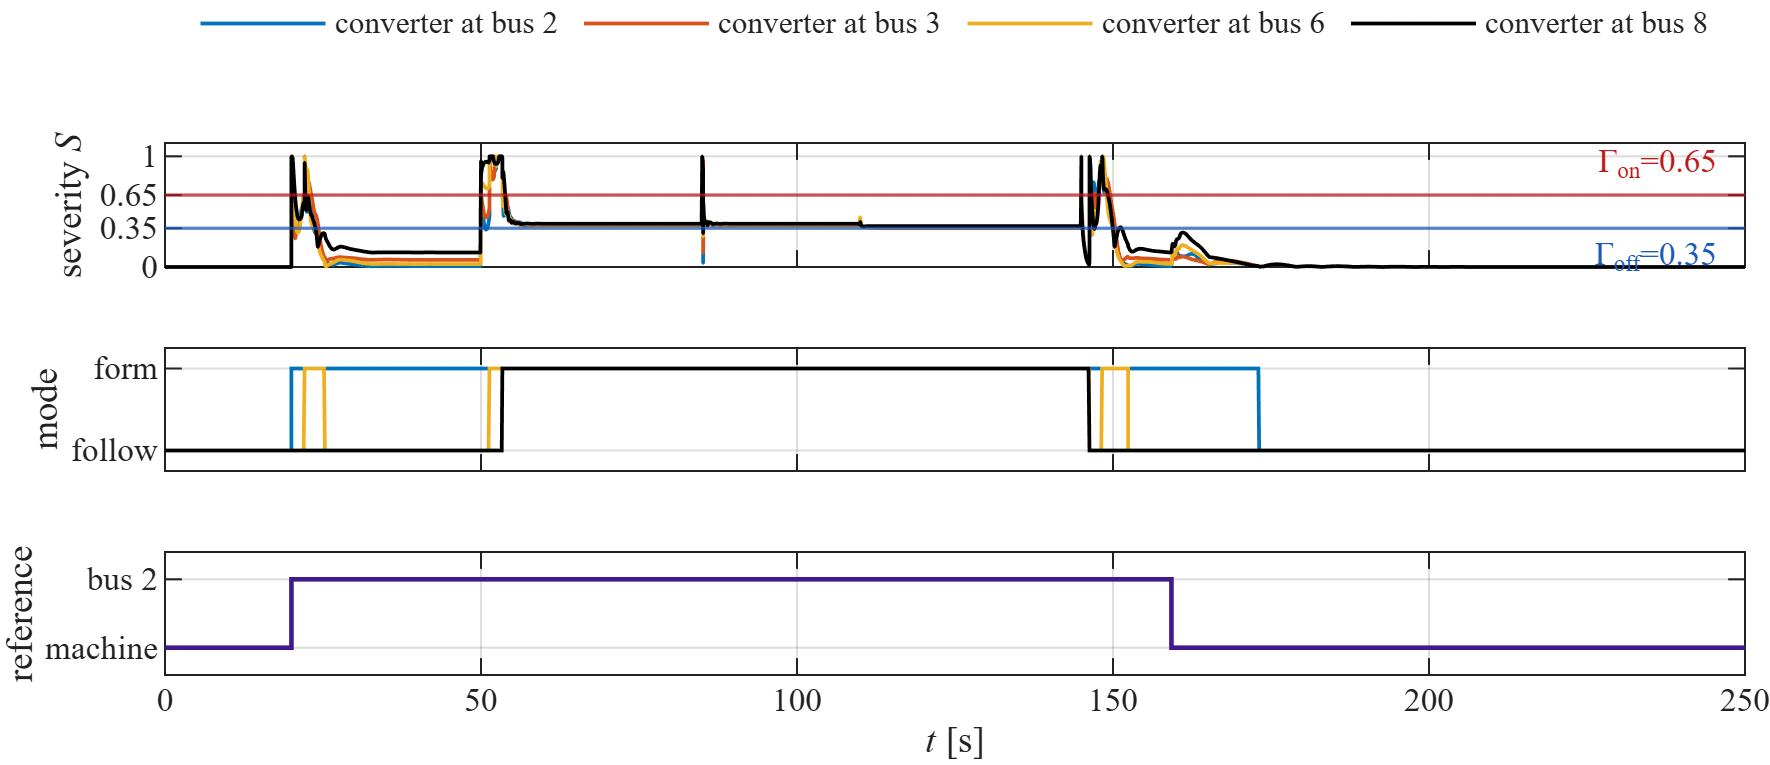
\includegraphics[width=\linewidth]{figures/presentation_pf_sssa_ts_gfm/slide_supervisor.png}
\end{columns}
\end{frame}

\begin{frame}{Result 3: Electrical Response}
\begin{columns}[c,onlytextwidth]
\column{0.34\textwidth}
\small
\begin{itemize}
  \item IBRs support the island after the SG trip.
  \item Frequency and voltage respond to each scheduled disturbance.
  \item The SG is reconnected only after the synchronism conditions are satisfied.
  \item The accepted run reaches the full $250$ s horizon.
\end{itemize}
\column{0.63\textwidth}
\centering
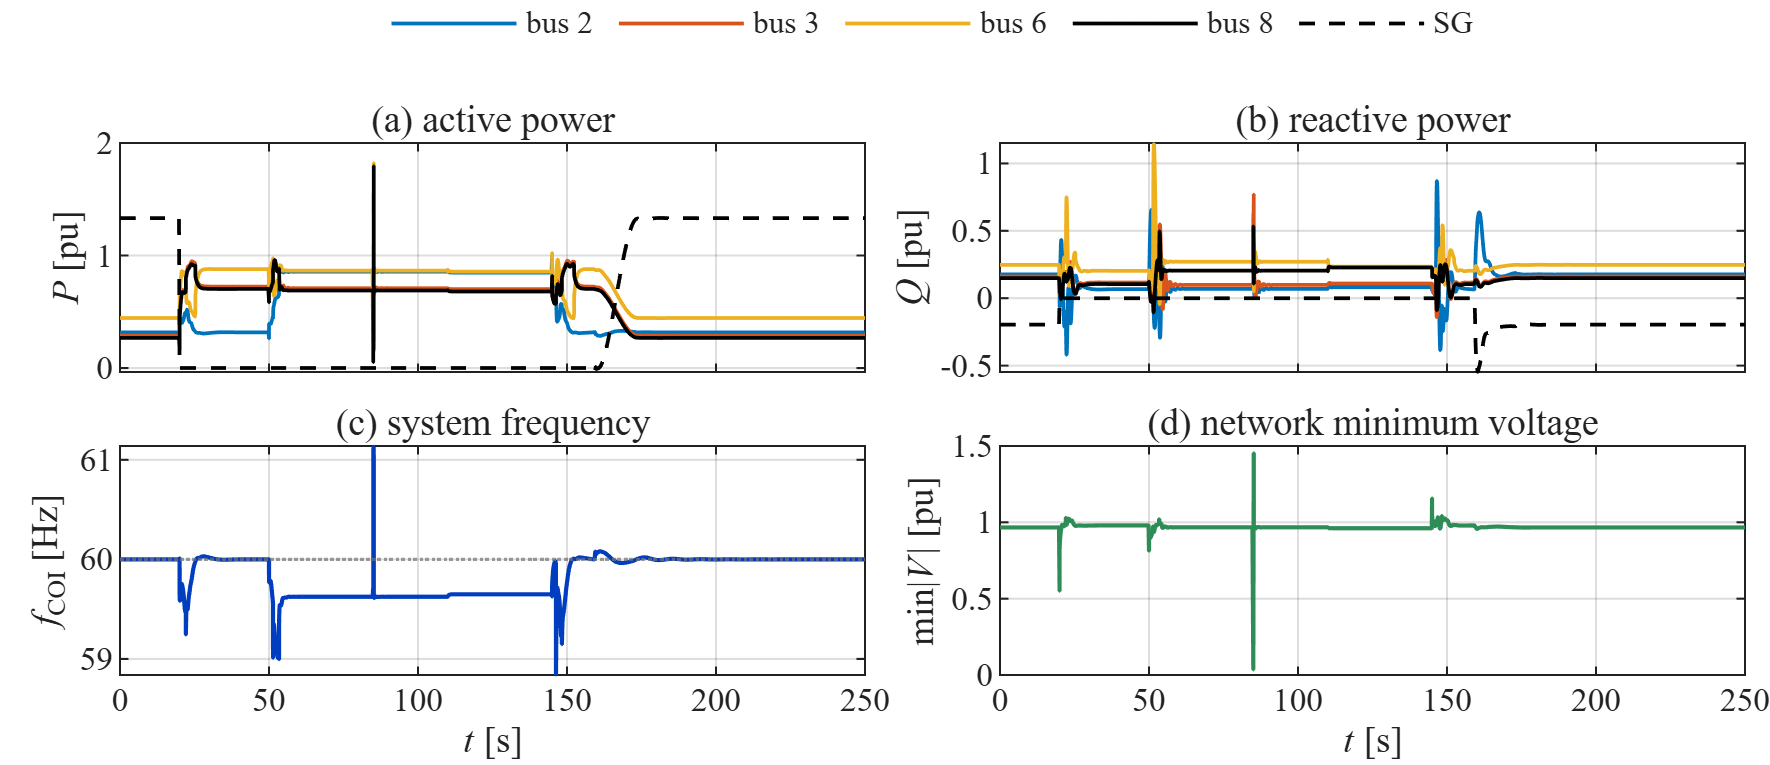
\includegraphics[width=\linewidth]{figures/presentation_pf_sssa_ts_gfm/slide_electrical.png}
\end{columns}
\end{frame}
\begin{frame}{Result 4: Converter Response under Different Policies}
\begin{columns}[c,onlytextwidth]
\column{0.34\textwidth}
\small
\begin{itemize}
  \item Staged switching: solid lines
  \item One pinned GFM: dashed lines
  \item Two pinned GFMs: dash-dot lines
\end{itemize}
\vspace{0.25cm}
\begin{block}{Main observation}
The power-sharing trajectory depends strongly on which converters are forming the grid and on when each mode transition occurs.
\end{block}
\column{0.63\textwidth}
\centering
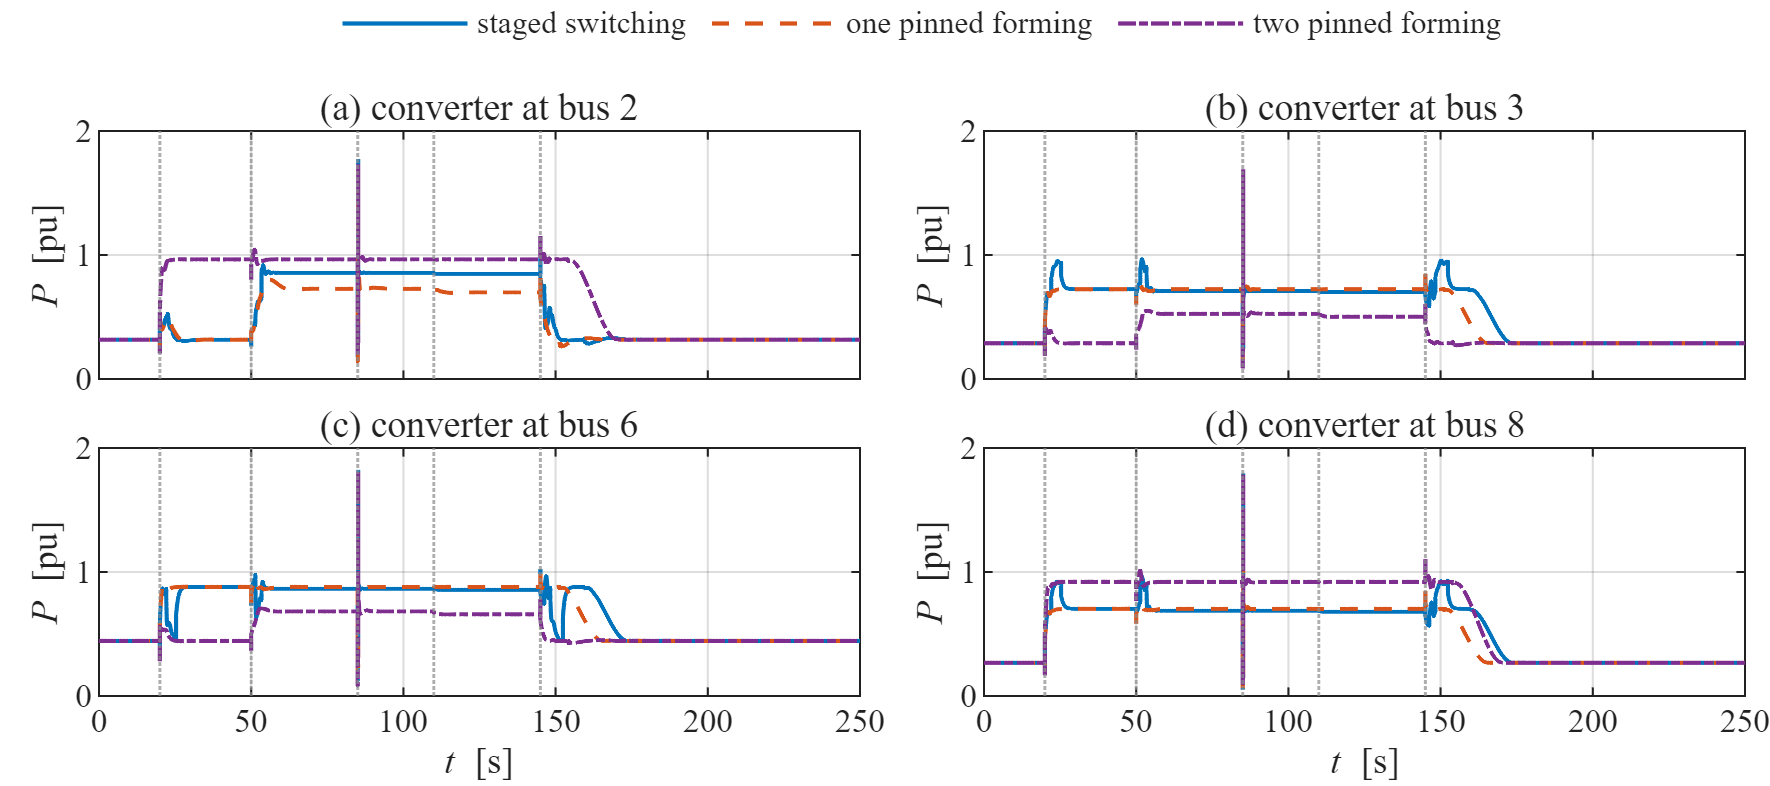
\includegraphics[width=\linewidth]{figures/presentation_pf_sssa_ts_gfm/slide_per_converter.png}
\end{columns}
\end{frame}

\section{Conclusion}
\begin{frame}{Conclusion}
\begin{columns}[c,onlytextwidth]
\column{0.58\textwidth}
\small
\begin{itemize}
  \item PF establishes the nonlinear operating point.
  \item SSSA screens candidate mode configurations around their equilibria.
  \item TS verifies the nonlinear trajectory through disturbances and switching.
  \item At least one GFM is required after the synchronous reference is lost.
  \item GFM admissibility is not monotonic with the number of forming units.
  \item Staged switching completes the $250$ s chronology and returns IBR support after SG recovery.
\end{itemize}
\column{0.39\textwidth}
\centering
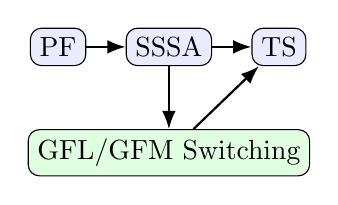
\begin{tikzpicture}[node distance=5mm,>=Latex]
\node[draw,rounded corners,fill=blue!8] (a) {PF};
\node[draw,rounded corners,fill=blue!8,right=of a] (b) {SSSA};
\node[draw,rounded corners,fill=blue!8,right=of b] (c) {TS};
\node[draw,rounded corners,fill=green!12,below=8mm of b] (d) {GFL/GFM Switching};
\draw[->,thick] (a)--(b); \draw[->,thick] (b)--(c); \draw[->,thick] (b)--(d); \draw[->,thick] (d)--(c);
\end{tikzpicture}
\vspace{0.35cm}
{\Large\bfseries Thank You}
\end{columns}
\end{frame}

\end{document}
